\documentclass{beamer}
%
% Choose how your presentation looks.
%
% For more themes, color themes and font themes, see:
% http://deic.uab.es/~iblanes/beamer_gallery/index_by_theme.html
%
\mode<presentation>
{
  \usetheme{Madrid}      % or try Darmstadt, Madrid, Warsaw, ...
  \usecolortheme{seahorse} % or try albatross, beaver, crane, ...
  \usefonttheme{serif}  % or try serif, structurebold, ...
  \setbeamertemplate{navigation symbols}{}
  \setbeamertemplate{caption}[numbered]
} 


\usepackage[english]{babel}
\usepackage{kotex}
%\usepackage[utf8x]{inputenc}

\title[게임수학 - 행렬]{ 게임 수학 강의 노트 04 - 행렬}
\author{강영민}
\institute{동명대학교}
\date{2015년 2학기}

\begin{document}

%%%%%%%%%%%%%%%%%%%%%%%%%%%%%%%%%%%%%%%%%%%%%%%%%%%%%%%%%
\begin{frame}
  \titlepage
\end{frame}

% Uncomment these lines for an automatically generated outline.
%\begin{frame}{Outline}
%  \tableofcontents
%\end{frame}


%%%%%%%%%%%%%%%%%%%%%%%%%%%%%%%%%%%%%%%%%%%%%%%%%%%%%%%%%


%%%%%%%%%%%%%%%%%%%%%%%%%%%%%%%%%%%%%%%%%%%%%%%%%%%%%%%%%
\begin{frame}{행렬}

\begin{itemize}
\item 행렬의 역사
	\begin{itemize}
	\item 1차 방정식의 풀이에 아주 오래 전부터 사용
	\item 그 특성이 정확히 파악되지 않고 1800년대까지는 배열(array)이라는 이름으로 알려짐
	\item 기원전 10세기에서 기원전 2세기 사이에 여러 세대에 걸쳐 쓰여진 중국의 구장산술(九章算術)에 연립 방정식을 풀기 위해 소개
	\item 판별식의 개념 등장
	\item 1545년에야 이탈리아 수학자 지롤라모 카르다노(Girolamo Cardano)가 그의 저서 "위대한 기술(Ars Magna)"를 통해 유럽에 전함
	\item 오랜 기간 동안 많은 수학자들이 이 행렬을 다루며 다양한 성질을 발견
	\item 행렬은 공간을 나루는 데에 필요한 유용한 도구
	\item 공간 내의 점들을 이떤 위치에서 다른 위치로 옮겨 놓는 다양한 변환이 행렬을 이용하여 표현됨
	\end{itemize}
\end{itemize}

\end{frame}


%%%%%%%%%%%%%%%%%%%%%%%%%%%%%%%%%%%%%%%%%%%%%%%%%%%%%%%%%


%%%%%%%%%%%%%%%%%%%%%%%%%%%%%%%%%%%%%%%%%%%%%%%%%%%%%%%%%
\begin{frame}{행렬이란 무엇인가}

\begin{itemize}
\item 행렬은 2차원으로 배열된 수
\item 가로 줄을 행(row), 세로 줄을 열(column)
\item $m$ 개의 행과 $n$ 개의 열로 이루어진 행렬은 $\mathbf A$는 다음의 모양
\item $\mathbf A = \left [ 
\begin{array}{cccccc}
a_{11} & a_{12} & \cdots & a_{1j} & \cdots & a_{1n} \\
a_{21} & a_{22} & \cdots & a_{2j} & \cdots & a_{2n} \\
\vdots & \vdots & \ddots &   \vdots   & \ddots & \vdots \\
a_{i1} & a_{i2} & \cdots & a_{ij} & \cdots & a_{in} \\
\vdots & \vdots & \ddots & \vdots & \ddots & \vdots\\
a_{m1} & a_{m2} & \cdots & a_{mj} & \cdots & a_{mn} \\
\end{array}
\right ]$
\item $m \times n$ 행렬이라고 하며 $\mathbf A \in \mathbb R^{m\times n}$로 표현
\item 각 행은 $n$ 개의 원소를 가진 행벡터(row vector)
\item 각 열은 $m$ 개의 원소를 가진 열벡터(column vector)
\end{itemize}

\end{frame}


%%%%%%%%%%%%%%%%%%%%%%%%%%%%%%%%%%%%%%%%%%%%%%%%%%%%%%%%%


%%%%%%%%%%%%%%%%%%%%%%%%%%%%%%%%%%%%%%%%%%%%%%%%%%%%%%%%%
\begin{frame}{행벡터와 열벡터}
$\mathbf A$를 행벡터 $\mathbf v_i^r$로 표현하면 다음과 같다.
$\mathbf A = \left [ 
\begin{array}{c}
\mathbf v_1^r\\
\mathbf v_2^r\\
\vdots\\
\mathbf v_m^r
\end{array}
\right ]$

$\mathbf A$를 열벡터 $\mathbf v_j^c$로 표현하면 다음과 같다.
$\mathbf A = \left [ 
\begin{array}{cccc}
\mathbf v_1^c & \mathbf v_2^c & \cdots & \mathbf v_n^c
\end{array}
\right ]$

\begin{figure}
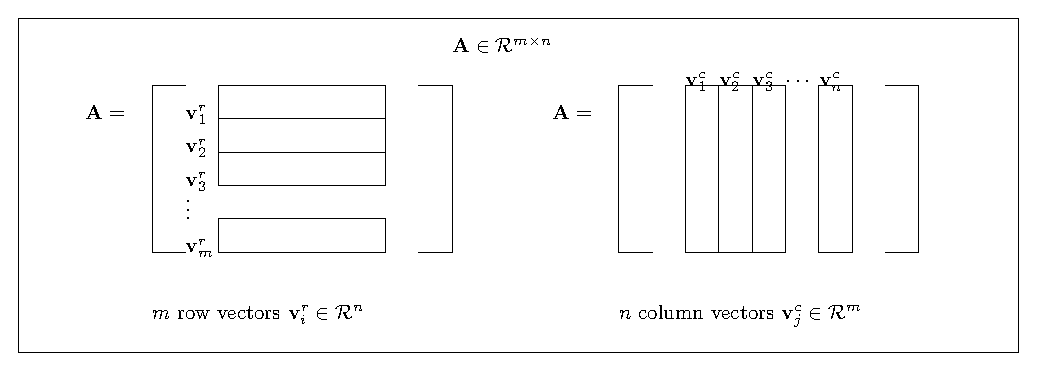
\includegraphics[width=12cm]{Math_matrix/matrixAsVectorCollection.eps}
\end{figure}

\end{frame}
%%%%%%%%%%%%%%%%%%%%%%%%%%%%%%%%%%%%%%%%%%%%%%%%%%%%%%%%%


%%%%%%%%%%%%%%%%%%%%%%%%%%%%%%%%%%%%%%%%%%%%%%%%%%%%%%%%%
\begin{frame}{정사각 행렬 - square matrix}

\begin{itemize}
\item 정방행렬, 혹은 정사각형 행렬은 행과 열의 수가 동일한 행렬.
	\begin{itemize}
	\item $\mathbf A \in \mathbb R^{n \times n}$인 행렬
	\item 정방행렬은 물리 문제에서 운동을 다루거나 그래픽스에서 변환을 다룰 때에 빈번히 나타남
	\end{itemize}
\item 다음 행렬 $\mathbf A$는 $3\times 3$의 정사각 행렬이다.
	\begin{itemize}
	\item $ \mathbf A = \left [ 
		\begin{array}{ccc}
		a_{11} & a_{12} & a_{13} \nonumber \\
		a_{21} & a_{22} & a_{23} \\
		a_{31} & a_{32} & a_{33} 
		\end{array}
		\right ] $
	\end{itemize}
\end{itemize}


\end{frame}
%%%%%%%%%%%%%%%%%%%%%%%%%%%%%%%%%%%%%%%%%%%%%%%%%%%%%%%%%


%%%%%%%%%%%%%%%%%%%%%%%%%%%%%%%%%%%%%%%%%%%%%%%%%%%%%%%%%
\begin{frame}{전치 행렬 - transpose}

\begin{itemize}
\item 어떤 행렬 $\mathbf A$의 전치행렬은 $\mathbf A^{\rm T}$
	\begin{itemize}
	\item $\mathbf B = \mathbf A^{\rm T} \Rightarrow b_{ij} = a_{ji}$
	\item 따라서, $m \times n$ 행렬의 전치는 $n \times m$ 행렬
	\item $\mathbf A \in \mathbb R^{m \times n} \Rightarrow \mathbf B \in \mathbb R^{n \times m}$
	\end{itemize}
\item 전치행렬의 성질
	\begin{itemize}
	\item $\mathbf (\mathbf A^{\rm T})^{\rm T} = A$
	\item $(\mathbf A + \mathbf B)^{\rm T} = \mathbf A^{\rm T} + \mathbf B^{\rm T}$
	\item $(k\mathbf A)^{\rm T} = k \mathbf A^{\rm T}$
	\item $(\mathbf {AB})^{\rm T} = \mathbf B^{\rm T} \mathbf A^{\rm T}$
	\end{itemize}
\item 그래픽스(graphics) 분야에서 매우 유용한 사용 방법은 회전 변환 행렬의 역행렬을 구할 때
\item 3차원 공간의 회전 변환은 정규직교(orthonormal) 특성
\item 정규직교 행렬의 역행렬은 그 행렬의 전치임이 알려져 있음
\end{itemize}

\end{frame}
%%%%%%%%%%%%%%%%%%%%%%%%%%%%%%%%%%%%%%%%%%%%%%%%%%%%%%%%%


%%%%%%%%%%%%%%%%%%%%%%%%%%%%%%%%%%%%%%%%%%%%%%%%%%%%%%%%%
\begin{frame}{대각 행렬 - diagonal matrix}

\begin{itemize}
\item 대각성분은 어떤 행렬 $\mathbf A$의 $i$ 행 $j$ 열 성분을 $a_{ij}$라고 표현할 때, $i=j$인 성분
\item 대각행렬은 대각성분을 제외한 다른 모든 성분의 값이 0인 행렬이다
	\begin{itemize}
	\item $\mathbf A = \left [ 
		\begin{array}{ccc}
		a_{11} & 0 & 0 \\
		0 & a_{22} & 0 \\
		0 & 0 & a_{33} \\
		\end{array}
		\right ]$
	\end{itemize}
\item 대각행렬을 다른 행렬과 곱했을 때의 성질
	\begin{itemize}
	\item 어떤 $3 \times 3$ 대각행렬을 $\mathbf D$, 1,2,3 행 대각성분은 $d_1, d_2, d_3$
	\item 다른 어떤 $3 \times 3$ 행렬 $\mathbf A$와 $\mathbf D$의 곱
		\begin{itemize}
		\item $\mathbf{DA} = \left [
			\begin{array}{ccc}
			d_1 a_{11} & d_1 a_{12} & d_1 a_{13} \\
			d_2 a_{21} & d_2 b_{22} & d_2 b_{23} \\
			d_3 a_{31} & d_3 b_{32} & d_3 b_{33} 
			\end{array}
			\right ]$
		\item 
		\item $\mathbf{AD} = \left [
			\begin{array}{ccc}
			d_1 a_{11} & d_2 a_{12} & d_3 a_{13} \\
			d_1 a_{21} & d_2 b_{22} & d_3 b_{23} \\
			d_1 a_{31} & d_2 b_{32} & d_3 b_{33}
			\end{array}
			\right ]$
		\end{itemize}
	\end{itemize}
\end{itemize}

\end{frame}
%%%%%%%%%%%%%%%%%%%%%%%%%%%%%%%%%%%%%%%%%%%%%%%%%%%%%%%%%


%%%%%%%%%%%%%%%%%%%%%%%%%%%%%%%%%%%%%%%%%%%%%%%%%%%%%%%%%
\begin{frame}{대각 행렬과 벡터의 곱 (1/2)}

대각행렬 $\mathbf D$와 열벡터 $\mathbf v \in \mathbb R^3$이 $(v_1, v_2, v_3)^{\rm T}$의 곱
$$
\mathbf {Dv} = 
\left [ 
\begin{array}{ccc}
a_{11} & 0 & 0 \\
0 & a_{22} & 0 \\
0 & 0 & a_{33} \\
\end{array}
\right ]
\left [
\begin{array}{c}
v_1 \\
v_2 \\
v_3 \\
\end{array}
\right ]
=
\left [
\begin{array}{c}
d_1 v_1 \\
d_2 v_2 \\
d_3 v_3 \\
\end{array}
\right ]
$$
\end{frame}
%%%%%%%%%%%%%%%%%%%%%%%%%%%%%%%%%%%%%%%%%%%%%%%%%%%%%%%%%


%%%%%%%%%%%%%%%%%%%%%%%%%%%%%%%%%%%%%%%%%%%%%%%%%%%%%%%%%
\begin{frame}{대각 행렬과 벡터의 곱 (2/2)}

행벡터 $\mathbf v^{\rm T}$와 대각행렬의 곱

$$
\mathbf v^{\rm T} \mathbf D = 
\left [
\begin{array}{ccc}
v_1 & v_2 & v_3 \\
\end{array}
\right ]
\left [ 
\begin{array}{ccc}
a_{11} & 0 & 0 \\
0 & a_{22} & 0 \\
0 & 0 & a_{33} \\
\end{array}
\right ]
=
\left [
\begin{array}{ccc}
d_1 v_1 & d_2 v_2 &d_3 v_3 \\
\end{array}
\right ]
$$

\end{frame}
%%%%%%%%%%%%%%%%%%%%%%%%%%%%%%%%%%%%%%%%%%%%%%%%%%%%%%%%%


%%%%%%%%%%%%%%%%%%%%%%%%%%%%%%%%%%%%%%%%%%%%%%%%%%%%%%%%%
\begin{frame}{행렬의 덧셈과 뺄셈}

두 행렬의 덧셈과 뺄셈은 동일한 크기의 행렬 사이에 정의됨

$$\mathbf A \in \mathbb R^{m \times n}  \wedge \mathbf A + \mathbf B = \mathbf C \Rightarrow \mathbf B, \mathbf C \in \mathbb R^{m \times n}$$
$$\mathbf A \in \mathbb R^{m \times n}  \wedge \mathbf A - \mathbf B = \mathbf D \Rightarrow \mathbf B, \mathbf D \in \mathbb R^{m \times n}$$

행렬과 덧셈과 뺄셈은 동일한 행과 열에 있는 성분을 서로 더하고, 빼서 원래의 자리에 기록

$$\mathbf A + \mathbf B = \mathbf C \Rightarrow c_{ij} = a_{ij} + b_{ij}$$
$$\mathbf A - \mathbf B = \mathbf D \Rightarrow d_{ij} = a_{ij} - b_{ij}$$

\end{frame}
%%%%%%%%%%%%%%%%%%%%%%%%%%%%%%%%%%%%%%%%%%%%%%%%%%%%%%%%%

%%%%%%%%%%%%%%%%%%%%%%%%%%%%%%%%%%%%%%%%%%%%%%%%%%%%%%%%%
\begin{frame}{행렬의 곱셈}

\begin{itemize}
\item $\mathbf A \in \mathbb R^{m \times n}$,  $\mathbf B \in \mathbb R^{n \times x}$
	\begin{itemize}
	\item $\mathbf {AB} = \mathbf C \in \mathbb R^{m \times x}$
	\end{itemize}
\end{itemize}

\begin{itemize}
\item $\mathbf A$의 앞에 $\mathbf B$를 곱할 경우
	\begin{itemize}
	\item $\mathbf B \in \mathbb R^{x \times m}$이어야 함
	\item 그 결과는 $\mathbf {BA} = \mathbf D \in \mathbb R^{x \times n}$
	\end{itemize}
\end{itemize}

\begin{itemize}
\item $\mathbf A \in \mathbb R^{m \times n}$, $\mathbf B \in \mathbb R^{n \times x}$
\item $\mathbf {AB} = \mathbf C \in \mathbb R^{m \times x}$
	\begin{itemize}
	\item $c_{ij}  =  a_{i1}b_{1j} + a_{i2}b_{2j} + \cdots + a_{in}b_{nj} $
	\item $c_{ij}  = \sum_{k=1}^n a_{ik} b_{kj}$
	\end{itemize}
\end{itemize}

행렬 $\mathbf A$의 $i$ 번째 행 벡터를 $\mathbf A_{i,*}$라고 하고, $j$ 번째 열 벡터를 $\mathbf B_{*,j}$라고 하면,
위의 식은 다음과 같이 다시 쓸 수 있다.

\begin{eqnarray}
c_{ij} & =  & \mathbf A_{i,*}^{\rm T} \cdot \mathbf B_{*,j}
\end{eqnarray}

\end{frame}
%%%%%%%%%%%%%%%%%%%%%%%%%%%%%%%%%%%%%%%%%%%%%%%%%%%%%%%%%


%%%%%%%%%%%%%%%%%%%%%%%%%%%%%%%%%%%%%%%%%%%%%%%%%%%%%%%%%
\begin{frame}{행렬과 스칼라의 곱}

행렬에 스칼라를 곱하는 연산은 해당 스칼라 값을 행렬의 모든 원소에 곱하면 된다.

$$k \mathbf A  = \mathbf B \Rightarrow b_{ij} = k a_{ij}$$

\end{frame}
%%%%%%%%%%%%%%%%%%%%%%%%%%%%%%%%%%%%%%%%%%%%%%%%%%%%%%%%%

%%%%%%%%%%%%%%%%%%%%%%%%%%%%%%%%%%%%%%%%%%%%%%%%%%%%%%%%%
\begin{frame}{행렬 덧셈과 뺄셈의 연산 법칙}

행렬은 다음과 같은 연산 법칙을 가진다.

\subsubsection{덧셈}

$$\mathbf A + \mathbf B = \mathbf B + \mathbf A$$
$$(\mathbf A + \mathbf B ) + \mathbf C = \mathbf A + ( \mathbf B + \mathbf C ) $$
$$ \mathbf A + 0 = 0 + \mathbf A = \mathbf A$$
$$ \mathbf A + (- \mathbf A ) = 0$$

이때, 0은 $\mathbf A$와 같은 차원의 행렬로 모든 원소가 0인 행렬이다.

\end{frame}
%%%%%%%%%%%%%%%%%%%%%%%%%%%%%%%%%%%%%%%%%%%%%%%%%%%%%%%%%


%%%%%%%%%%%%%%%%%%%%%%%%%%%%%%%%%%%%%%%%%%%%%%%%%%%%%%%%%
\begin{frame}{행렬 스칼라 곱의 연산 법칙}

$$(k+l) \mathbf A = k \mathbf A + l \mathbf A$$
$$k (\mathbf A + \mathbf B ) = k \mathbf A + k \mathbf B$$
$$(kl) \mathbf A = k (l \mathbf A)$$
$$ (-1) \mathbf A = -\mathbf A$$
$$ 0 \mathbf A = 0$$


\end{frame}
%%%%%%%%%%%%%%%%%%%%%%%%%%%%%%%%%%%%%%%%%%%%%%%%%%%%%%%%%

%%%%%%%%%%%%%%%%%%%%%%%%%%%%%%%%%%%%%%%%%%%%%%%%%%%%%%%%%
\begin{frame}{행렬 곱셈의 연산 법칙}

$$\mathbf{AB} \neq \mathbf {BA}$$
$$\mathbf{A(BC)} = \mathbf{(AB)C}$$
$$\mathbf{A(B+C)} = \mathbf {AB} + \mathbf {AC}$$
$$\mathbf{(A+B)C} = \mathbf{AC} + \mathbf{BC}$$
$$\mathbf{AI} = \mathbf{IA} = \mathbf A$$
$$k \mathbf{AB} = (k\mathbf A)\mathbf B = \mathbf A k \mathbf B$$

$\mathbf I$는 항등행렬

\end{frame}
%%%%%%%%%%%%%%%%%%%%%%%%%%%%%%%%%%%%%%%%%%%%%%%%%%%%%%%%%

%%%%%%%%%%%%%%%%%%%%%%%%%%%%%%%%%%%%%%%%%%%%%%%%%%%%%%%%%
\begin{frame}{행렬식 1/2}

\begin{itemize}
\item 행렬식은 정방행렬에서 정의된다.
\item 어떤 행렬 $\mathbf A$의 행렬식은 $det \mathbf A$, $det(\mathbf A)$, 또는 $|\mathbf A|$로 표현
\item 행렬식을 계산하기 위해 필요한 개념
	\begin{itemize}
	\item 소행렬식(minor)
	\item 여인자(cofactor)
	\end{itemize}
\item 소행렬식
	\begin{itemize}
	\item $\mathbf A \in \mathbb R^{m \times n}$: 이 행렬은 $m \times n$개의 소행렬식(minor) $M_{ij}$를 가짐
	\item 각 $M_{ij}$는 $\mathbf A$ 행렬의 $i$ 행 벡터 전체와 $j$ 열 벡터 전체를 제거하고 얻어지는 행렬($\in \mathbb R^{m-1 \times n-1}$)의 
행렬식
	\end{itemize}
\item 여인자
	\begin{itemize}
	\item 행렬 $\mathbf A$의 여인자는 소행렬식이 구해지는 위치마다 결정
	\item 다음과 같이 정의되는 $m \times n$개의 여인자 $C_{ij}$가 존재
	\item $C_{ij} = (-1)^{i+j} M_{ij}$
	\end{itemize}
\end{itemize}

\end{frame}
%%%%%%%%%%%%%%%%%%%%%%%%%%%%%%%%%%%%%%%%%%%%%%%%%%%%%%%%%


%%%%%%%%%%%%%%%%%%%%%%%%%%%%%%%%%%%%%%%%%%%%%%%%%%%%%%%%%
\begin{frame}{행렬식 2/2}

\begin{itemize}
\item 행렬 $\mathbf A \in \mathbb R^{m \times n}$의 $i$ 행, $j$ 열 여인자 $C_{ij}$를 이용한 행렬식 계산
\end{itemize}
\begin{eqnarray}
det \mathbf A &= | \mathbf A | &= \sum_{j=1}^n A_{1j} C_{1j} = \sum_{j=1}^n A_{2j} C_{2j} = \cdots = \sum_{j=1}^n A_{mj} C_{mj} \\ \nonumber
& &= \sum_{i=1}^m A_{i1} C_{i1} = \sum_{i=1}^m A_{i2} C_{i2} = \cdots = \sum_{j=1}^n A_{in} C_{in} 
\end{eqnarray}

\begin{itemize}
\item $\mathbf A$의 임의의 행 벡터 $\mathbf A_{i,*}$와 $\mathbf C$의 동일 위치 행 벡터 $\mathbf C_{i,*}$의 내적
\item $\mathbf A$의 임의의 열 벡터 $\mathbf A_{*,j}$와 $\mathbf C$의 동일 위치 열 벡터 $\mathbf C_{*,j}$의 내적
\end{itemize}

\begin{eqnarray}
det \mathbf A = | \mathbf A | = \mathbf A_{i,*} \mathbf C_{i,*}^{\rm T} = \mathbf A_{*,j}^{\rm T} \mathbf C_{*,j}
\end{eqnarray}

\end{frame}
%%%%%%%%%%%%%%%%%%%%%%%%%%%%%%%%%%%%%%%%%%%%%%%%%%%%%%%%%


%%%%%%%%%%%%%%%%%%%%%%%%%%%%%%%%%%%%%%%%%%%%%%%%%%%%%%%%%
\begin{frame}{예제}
\hrule

\noindent \colorbox{lightgray}{\begin{minipage}{6cm}예제\end{minipage}} 


\noindent  다음 행렬의 행렬식을 구하라.
$
\left [
\begin{array}{cc}
A_{11} & A_{12} \\
A_{21} & A_{22}
\end{array}
\right ]
$

\noindent \colorbox{lightgray}{\begin{minipage}{6cm}정답\end{minipage}} 

여인자 $M_{ij}$를 구한다.
$$
\mathbf M = 
\left [
\begin{array}{cc}
M_{11} & M_{12} \\
M_{21} & M_{22}
\end{array}
\right ] = 
\left [
\begin{array}{cc}
det \left [ A_{22} \right ] &
det \left [ A_{21} \right ] \\
det \left [ A_{12} \right ] &
det \left [ A_{11} \right ] 
\end{array}
\right ]
= 
\left [
\begin{array}{cc}
A_{22} & A_{21} \\
A_{12} & A_{11} 
\end{array}
\right ]
$$

여인자의 정의에 따라, 여인자로 구성된 행렬 $\mathbf C$는 다음과 같다.
$$
\mathbf C = 
\left [
\begin{array}{cc}
(-1)^{1+1} A_{22} & (-1)^{1+2} A_{21} \\
(-1)^{2+1} A_{12} & (-1)^{2+2} A_{11} 
\end{array}
\right ]
= \left [
\begin{array}{cc}
A_{22} & -A_{21} \\
-A_{12} & A_{11} 
\end{array}
\right ]
$$

$\mathbf A$의 임의의 행 벡터를 선택할 수 있으므로 우선 1행을 가지고 오자. 그리고 여인자 행렬 $\mathbf C$의 1행을 가지고 와서, 두 행 벡터의 내적을 
구하면 다음과 같다.
$$det \mathbf A  = \mathbf A_{1,*}  \mathbf C_{1,*}^{\rm T}  =  A_{11}  A_{22} +  A_{12} (-  A_{21}) $$

\hrule
\end{frame}
%%%%%%%%%%%%%%%%%%%%%%%%%%%%%%%%%%%%%%%%%%%%%%%%%%%%%%%%%

%%%%%%%%%%%%%%%%%%%%%%%%%%%%%%%%%%%%%%%%%%%%%%%%%%%%%%%%%
\begin{frame}{행렬식의 기하적 의미}

두 열 벡터 $\mathbf a = (a_x a_y )^{\rm T}$와 $\mathbf b = (b_x , b_y)^{\rm T}$를 열로 하는 행렬 $\mathbf A$
$$\mathbf A = \left [ 
\begin{array}{cc}
a_x & b_x \\
a_y & b_y
\end{array}
\right ]
$$
이 두 벡터를 두 개의 변으로 하는 평행사변형의 넓이가 행렬 $\mathbf A$의 행렬식



\begin{figure}
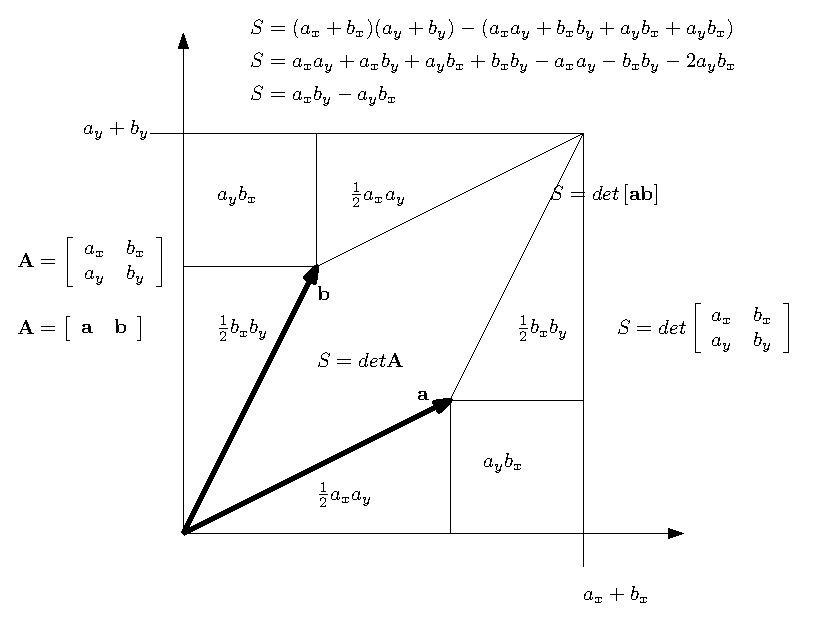
\includegraphics[width=7cm]{Math_matrix/determinantGeo.eps}
\end{figure}

\end{frame}
%%%%%%%%%%%%%%%%%%%%%%%%%%%%%%%%%%%%%%%%%%%%%%%%%%%%%%%%%


%%%%%%%%%%%%%%%%%%%%%%%%%%%%%%%%%%%%%%%%%%%%%%%%%%%%%%%%%
\begin{frame}{$3 \times 3$ 행렬의 행렬식 의미}

$\mathbf A \in \mathbb R^{3 \times 3}$는 세 개의 벡터 $\mathbf a, \mathbf b, \mathbf c$를 포함

$$
\mathbf A = \left [ \begin{array}{ccc}
a_1 & b_1 & c_1 \\
a_2 & b_2 & c_2 \\
a_3 & b_3 & c_3 
\end{array} \right ] =
\left [ \begin{array}{ccc}
\mathbf a & \mathbf b & \mathbf c
\end{array} \right ] 
$$

이 세 개의 벡터들이 만드는 평행육면체의 크기가 세 개의 벡터들로 구성된 행렬의 행렬식


\begin{figure}
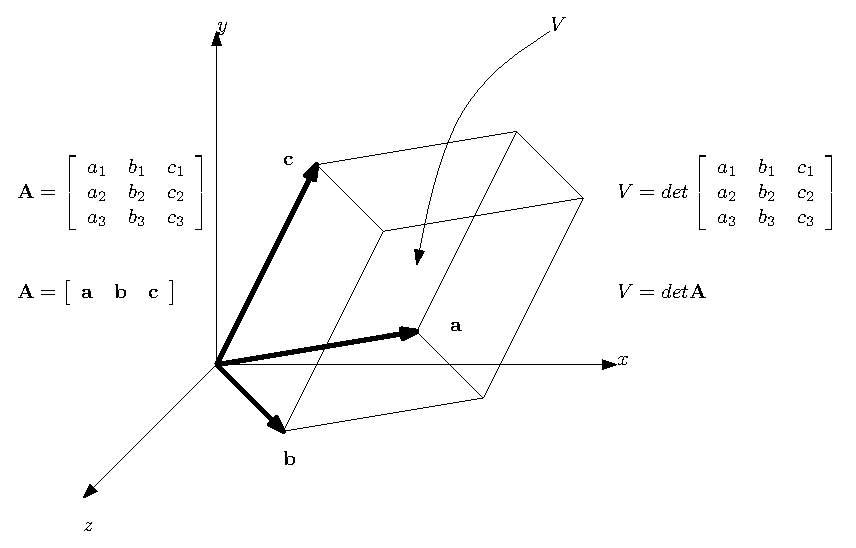
\includegraphics[width=7cm]{Math_matrix/determinantGeo3D.eps}
\end{figure}

\end{frame}
%%%%%%%%%%%%%%%%%%%%%%%%%%%%%%%%%%%%%%%%%%%%%%%%%%%%%%%%%


%%%%%%%%%%%%%%%%%%%%%%%%%%%%%%%%%%%%%%%%%%%%%%%%%%%%%%%%%
\begin{frame}{행렬과 행렬식의 기하적 의미}

\begin{figure}
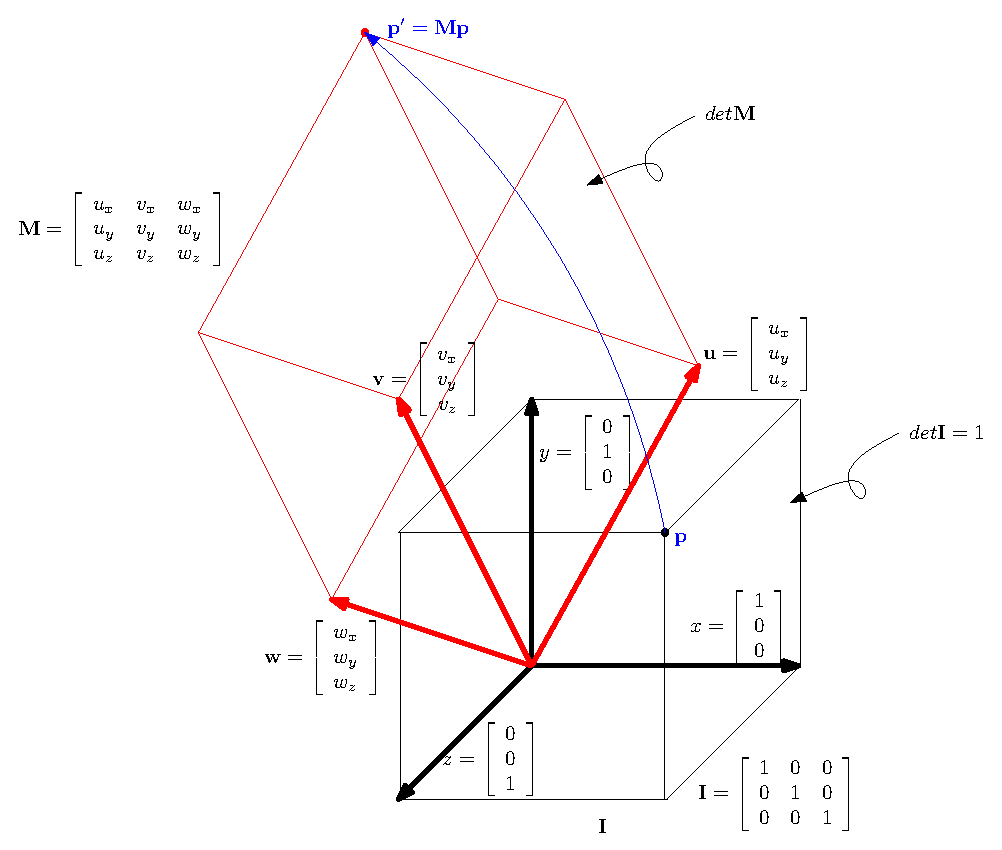
\includegraphics[width=8cm]{Math_matrix/matrixConcept.eps}
\end{figure}

\end{frame}
%%%%%%%%%%%%%%%%%%%%%%%%%%%%%%%%%%%%%%%%%%%%%%%%%%%%%%%%%

%%%%%%%%%%%%%%%%%%%%%%%%%%%%%%%%%%%%%%%%%%%%%%%%%%%%%%%%%
\begin{frame}{행렬식의 특성}

몇 가지 기억해 둘 행렬식의 특성은 다음과 같다.

$$|\mathbf A| = |\mathbf A^{\rm T}|$$

$$\mathbf A \in \mathbb R^{n \times n} \Rightarrow | k \mathbf A | = k^n |\mathbf A|$$

$$|\mathbf {AB}| = |\mathbf A| |\mathbf B|$$

\end{frame}
%%%%%%%%%%%%%%%%%%%%%%%%%%%%%%%%%%%%%%%%%%%%%%%%%%%%%%%%%

%%%%%%%%%%%%%%%%%%%%%%%%%%%%%%%%%%%%%%%%%%%%%%%%%%%%%%%%%
\begin{frame}{역행렬}


\begin{itemize}
\item 역행렬은 정방행렬에만 존재
\item $\mathbf A$의 역행렬이 존재한다면, 이 역행렬을 $\mathbf A^{-1}$로 표현
\item 역행렬 $\mathbf A^{-1}$은 다음과 같은 조건을 만족
	\begin{itemize}
	\item $\mathbf {AA}^{-1} = \mathbf I$
	\item $\mathbf A^{-1} \mathbf A = \mathbf I$
	\end{itemize}
\end{itemize}

\begin{itemize}
\item 역행렬이 존재하는 행렬을 가역행렬(invertible matrix)
\item 역행렬이 존재하지 않는 행렬은 특이행렬(singular matrix)
\end{itemize}

\begin{itemize}
\item 의사 역행렬(pseudo-inverse)
	\begin{itemize}
	\item  행렬 $\mathbf A$가 정방행렬이 아니고 $\mathbb R^{m \times n}$에 속한다고 하자. 다른 어떤 행렬 $\mathbf B$가 $\mathbb R^{n \times m}$에 속하면, 두 행렬의 곱 $\mathbf {AB}$는 $\mathbb R^{m \times m}$에 속하는 정방행렬이 된다. 만약 $\mathbf {AB} = \mathbf I \in \mathbb R^{n \times n}$이라면, $\mathbf B$를 $\mathbf A$의 의사 역행렬(pseudo-inverse)라고 한다.
	\end{itemize}
\end{itemize}
\end{frame}
%%%%%%%%%%%%%%%%%%%%%%%%%%%%%%%%%%%%%%%%%%%%%%%%%%%%%%%%%


%%%%%%%%%%%%%%%%%%%%%%%%%%%%%%%%%%%%%%%%%%%%%%%%%%%%%%%%%
\begin{frame}{역행렬의 계산}

\begin{itemize}
\item 역행렬의 계산은 수반행렬(adjoint matrix)를 이용하여 쉽게 정의
	\begin{itemize}
	\item 행렬 $\mathbf A$의 수반행렬: 여인자 $C_{ij}$를 성분으로 하는 행렬 $\mathbf C$의 전치(transpose)
	\end{itemize}
\end{itemize}


$$ adj \mathbf A = 
\left (
\begin{array}{cccc}
C_{11} & C_{21} & \cdots & C_{n1} \\
C_{12} & C_{22} & \cdots & C_{n2} \\
\vdots & \vdots & \ddots & \vdots \\
C_{1n} & C_{2n} & \cdots & C_{nn} \\
\end{array}
\right )
= \mathbf C^{\rm T}
$$
 
\begin{itemize}
\item 수반행렬을 행렬의 행렬식으로 나누면 역행렬이 된다.
\end{itemize}

$$\mathbf A^{-1} = \frac{adj \mathbf A}{|\mathbf A|} = 
\frac{1}{|\mathbf A|}
\left (
\begin{array}{cccc}
C_{11} & C_{21} & \cdots & C_{n1} \\
C_{21} & C_{22} & \cdots & C_{n2} \\
\vdots & \vdots & \ddots & \vdots \\
C_{n1} & C_{2n} & \cdots & C_{nn} \\
\end{array}
\right )
= \mathbf C^{\rm T}
$$

식은 간단하지만, 여인자를 구하는 재귀호출이 매우 많은 계산을 요구

\end{frame}
%%%%%%%%%%%%%%%%%%%%%%%%%%%%%%%%%%%%%%%%%%%%%%%%%%%%%%%%%


\end{document}


